Abbildung \ref{fig:aufbau} zeigt den prinzipiellen Aufbau des Versuchs
% \begin{figure}
  % \centering
  % 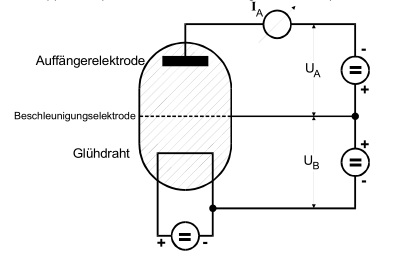
\includegraphics[width=0.7\textwidth]{bilder/aufbau.jpg}
  % \caption{prinzipieller Aufbau des Franck-Hertz-Versuchs \cite{601}}
  % \label{fig:aufbau}
% \end{figure}
Der Aufbau besteht aus einem Glasrohr, welches mit Hg-Dampf gefüllt ist,
sowie einem Heizfaden, einer Beschleunigungs- und einer Auffängerelektrode
die ebenfalls im Glasrohr untergebracht sind.
Das Glasrohr selbst befindet sich einem heizbaren Blechgehäuse, dessen
Innentemperatur $\su{T}$ mit einem elektrischen Temperaturreglers konstant
gehalten wird. Die Temperatur wird mit einem Thermometer abgelesen.

Der Glühfaden wird durch ein seperates Konstantspannungsgerät versorgt, welches
sich präzise einstellen lässt. Beschleunigungs- und Bremsspannung werden von
zwei elektronischen Geräten geliefert, deren Ausgangsspannung sich
zeitproportional ändern kann. Der Auffängerstrom wird auf seiner geringen Größe
mit einem Picoamperemeter gemessen. Hierbei handelt es sich um einen
Gleichstromverstärker mit eingebautem Amperemeter, dessen Ausschlag proportional
zum zum Eingangsstrom ist.
